%----------------------------------------------------------------------------------------
%	PACKAGES AND OTHER DOCUMENT CONFIGURATIONS
%----------------------------------------------------------------------------------------

\documentclass[10pt, a4paper]{article} % 10pt font size (11 and 12 also possible), A4 paper (letterpaper for US letter) and two column layout (remove for one column)


%----------------------------------------------------------------------------------------
%	PACKAGES AND OTHER DOCUMENT CONFIGURATIONS
%----------------------------------------------------------------------------------------

\usepackage[english]{babel} % English language hyphenation

\usepackage{microtype} % Better typography

\usepackage{amsmath,amsfonts,amsthm} % Math packages for equations

\usepackage[svgnames]{xcolor} % Enabling colors by their 'svgnames'

\usepackage[hang, small, labelfont=bf, up, textfont=it]{caption} % Custom captions under/above tables and figures

\usepackage{booktabs} % Horizontal rules in tables

\usepackage{lastpage} % Used to determine the number of pages in the document (for "Page X of Total")

\usepackage{graphicx} % Required for adding images

\usepackage{enumitem} % Required for customising lists
\setlist{noitemsep} % Remove spacing between bullet/numbered list elements

\usepackage{sectsty} % Enables custom section titles
\allsectionsfont{\usefont{OT1}{phv}{b}{n}} % Change the font of all section commands (Helvetica)

\usepackage{bbm}

%----------------------------------------------------------------------------------------
%	MARGINS AND SPACING
%----------------------------------------------------------------------------------------

\usepackage{geometry} % Required for adjusting page dimensions

\geometry{
	top=1cm, % Top margin
	bottom=1.5cm, % Bottom margin
	left=2cm, % Left margin
	right=2cm, % Right margin
	includehead, % Include space for a header
	includefoot, % Include space for a footer
	%showframe, % Uncomment to show how the type block is set on the page
}

\setlength{\columnsep}{7mm} % Column separation width

%----------------------------------------------------------------------------------------
%	FONTS
%----------------------------------------------------------------------------------------

\usepackage[T1]{fontenc} % Output font encoding for international characters
\usepackage[utf8]{inputenc} % Required for inputting international characters

\usepackage{XCharter} % Use the XCharter font

%----------------------------------------------------------------------------------------
%	HEADERS AND FOOTERS
%----------------------------------------------------------------------------------------

\usepackage{fancyhdr} % Needed to define custom headers/footers
\pagestyle{fancy} % Enables the custom headers/footers

\renewcommand{\headrulewidth}{0.0pt} % No header rule
\renewcommand{\footrulewidth}{0.4pt} % Thin footer rule

\renewcommand{\sectionmark}[1]{\markboth{#1}{}} % Removes the section number from the header when \leftmark is used

%\nouppercase\leftmark % Add this to one of the lines below if you want a section title in the header/footer

% Headers
\lhead{} % Left header
\chead{\textit{\thetitle}} % Center header - currently printing the article title
\rhead{} % Right header

% Footers
\lfoot{} % Left footer
\cfoot{} % Center footer
\rfoot{\footnotesize Page \thepage\ of \pageref{LastPage}} % Right footer, "Page 1 of 2"

\fancypagestyle{firstpage}{ % Page style for the first page with the title
	\fancyhf{}
	\renewcommand{\footrulewidth}{0pt} % Suppress footer rule
}

%----------------------------------------------------------------------------------------
%	TITLE SECTION
%----------------------------------------------------------------------------------------

\newcommand{\authorstyle}[1]{{\large\usefont{OT1}{phv}{b}{n}\color{DarkRed}#1}} % Authors style (Helvetica)

\newcommand{\institution}[1]{{\footnotesize\usefont{OT1}{phv}{m}{sl}\color{Black}#1}} % Institutions style (Helvetica)

\usepackage{titling} % Allows custom title configuration

\newcommand{\HorRule}{\color{DarkGoldenrod}\rule{\linewidth}{1pt}} % Defines the gold horizontal rule around the title

\pretitle{
	\vspace{-30pt} % Move the entire title section up
	\HorRule\vspace{10pt} % Horizontal rule before the title
	\fontsize{20}{20}\usefont{OT1}{phv}{b}{n}\selectfont % Helvetica
	\color{DarkRed} % Text colour for the title and author(s)
}

\posttitle{\par\vskip 15pt} % Whitespace under the title

\preauthor{} % Anything that will appear before \author is printed

\postauthor{ % Anything that will appear after \author is printed
	\vspace{10pt} % Space before the rule
	\par\HorRule % Horizontal rule after the title
	\vspace{20pt} % Space after the title section
}

%----------------------------------------------------------------------------------------
%	ABSTRACT
%----------------------------------------------------------------------------------------

\usepackage{lettrine} % Package to accentuate the first letter of the text (lettrine)
\usepackage{fix-cm}	% Fixes the height of the lettrine

\newcommand{\initial}[1]{ % Defines the command and style for the lettrine
	\lettrine[lines=3,findent=4pt,nindent=0pt]{% Lettrine takes up 3 lines, the text to the right of it is indented 4pt and further indenting of lines 2+ is stopped
		\color{DarkGoldenrod}% Lettrine colour
		{#1}% The letter
	}{}%
}

\usepackage{xstring} % Required for string manipulation

\newcommand{\lettrineabstract}[1]{
	\StrLeft{#1}{1}[\firstletter] % Capture the first letter of the abstract for the lettrine
	\initial{\firstletter}\textbf{\StrGobbleLeft{#1}{1}} % Print the abstract with the first letter as a lettrine and the rest in bold
}

%----------------------------------------------------------------------------------------
%	BIBLIOGRAPHY
%----------------------------------------------------------------------------------------

\usepackage[backend=bibtex,natbib=true]{biblatex} % Use the bibtex backend with the authoryear citation style (which resembles APA)

\addbibresource{bibl.bib} % The filename of the bibliography

\usepackage[autostyle=true]{csquotes} % Required to generate language-dependent quotes in the bibliography
 % Specifies the document structure and loads requires packages

%----------------------------------------------------------------------------------------
%	ARTICLE INFORMATION
%----------------------------------------------------------------------------------------

\title{Estimation of the Probability of Successful Transmission of Uplink Messages in LoRaWAN} % The article title

\author{
	\authorstyle{Ante Lojić Kapetanović}
	\newline\newline % Space before institutions
	\institution{University of Split, Split, Croatia}
}

% Example of a one line author/institution relationship
%\author{\newauthor{John Marston} \newinstitution{Universidad Nacional Autónoma de México, Mexico City, Mexico}}

\date{\today} % Add a date here if you would like one to appear underneath the title block, use \today for the current date, leave empty for no date

%----------------------------------------------------------------------------------------

\begin{document}

\maketitle % Print the title

\thispagestyle{firstpage} % Apply the page style for the first page (no headers and footers)

%----------------------------------------------------------------------------------------
%	ABSTRACT
%----------------------------------------------------------------------------------------

\lettrineabstract{This report is a short overview of applying forecasting methods on data from real LoRaWAN deployment in Svebølle, Denmark. The main idea is to examine whether there is a possibility of predicting successful transmission of LoRa messages for the given future time interval. Proposed model for prediction is Long Short-Term Memory (LSTM), an artificial recurrent neural network (RNN) architecture used in the field of deep learning.}

%----------------------------------------------------------------------------------------
%	ARTICLE CONTENTS
%----------------------------------------------------------------------------------------

\section{Introduction}
TBA

\section{Network Topology}

LoRaWAN - Long Range Wide Area Network - low power, wide area media access protocol designed to wirelessly connect 'things' to the internet. LoRaWAN is useful in IoT deployment, specially in smart environments where there are thousands of end-devices (i.e. sensors) that require minimal bandwidth and minimal energy.

The network architecutre is deployed in a star-of-stars topology in which gateways relay messages between end-devices and a central network server \cite{Silva_LoRaWAN}.
Toplogy overview is shown in Fig. \ref{lorawan}.
\begin{figure}
	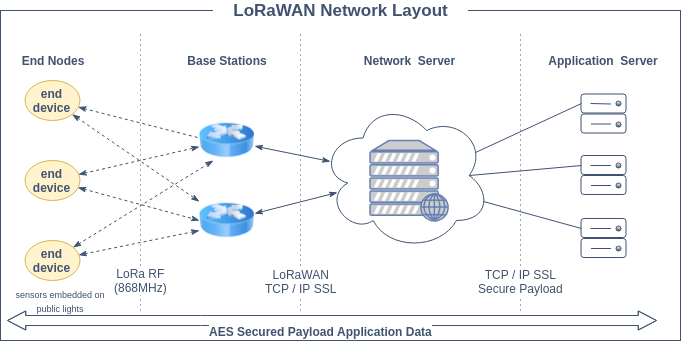
\includegraphics[width=\linewidth]{images/LoRaWAN-Network-Layout.png} % Figure image
	\caption{LoRaWAN Network Layout} % Figure caption
	\label{lorawan} % Label for referencing with \ref{bear}
\end{figure}


End-device is transmitting data to base station using LoRa technology, which means that data is modulated using CSS technique and transmitted using 868MHz RF, also it is worth mentioning that data is encrypted using AES128 in Counter mode (CTR). If the packet’s FPort is set to 0 then the NwkSKey is used, otherwise the AppSKey is used. An important feature of all messages in LoRa is that the counters for sent (FCntUp) and received (FCntDown) messages are maintained by the Node and Network Server, and that these counters never repeat \cite{Miller_LoRaSecurity}.
base stations relay messages from end-nodes to network server using a back-haul wireless network with higher frequency (often 2.4GHz) or using wired connection (Ethernet, optics). 
Network server decodes the packets received from base station and performs security checks and adaptive data rate so it can generate the packets that should be sent back to end-devices \cite{Silva_LoRaWAN}.

Observed LoRaWAN network model deployed in Svebølle is consisted of a single base station which communicates with few hundreds of different end-devices; network topology is quite simple and shown on Fig. \ref{svebolle}.
\begin{figure}
	\centering
	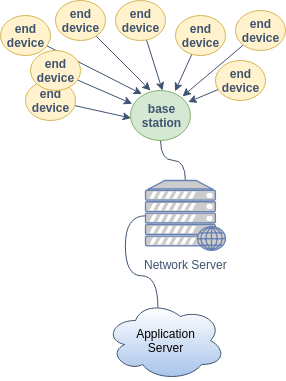
\includegraphics[scale=.7]{images/Svebolle-Topology.png} % Figure image
	\caption{Overview of Svebølle LoRaWAN network} % Figure caption
	\label{svebolle} 
\end{figure}

Data was collected during the period of 4 months and 14 days, during which approximately 689 thousands measurements were generated and captured. 
There is only one base station and, judgdin by the exploration of the data set, 251 end-devices in the network.
Measurements were carried out on the base station side and there are more than few relevant labels:
\begin{itemize}
	\item Time - basic datetime format to microsecond precision
    \item DevAddr - device address written as HEX string
    \item Freq - carrier signal radio frequency
    \item Chan - channel number
    \item BW - bandwidth
    \item SPF - spreading factor
    \item RSSI - received signal strength indication
    \item SNR - Signal-to-Noise ratio
    \item CR - code rate 
    \item DR - data rate
    \item crcStatus - cyclic redundancy check
    \item mType - type of MAC message
    \item macPayload - part of transmitted data that is the actual intended message
    \item id - packet identification
\end{itemize}

All of these indicators are described in details in \cite{Aloys_LoRa}.

Considering the data, simple communication model of this LoRaWAN network could be deduced and is shown in Fig. \ref{communication}
\begin{figure}
	\centering
	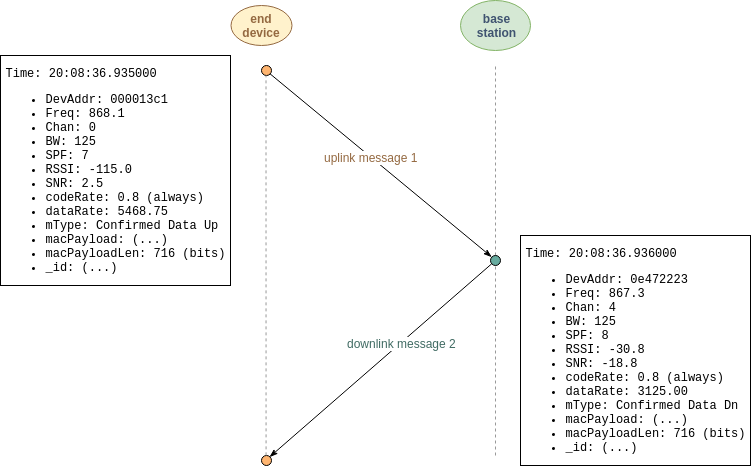
\includegraphics[scale=.5]{images/Svebolle-ed-bs-model.png} % Figure image
	\caption{Communication between end-device and base station in LoRaWAN network in Svebølle} % Figure caption
	\label{communication} 
\end{figure}

\section{Introducing the Idea of ANN}

Measurements in data set were not structured as time-series data, only times when transmission of LoRa message actually happend in uplink direction are captured and stored. 
Time series data is a series of data points indexed in time order and taken at successive equally spaced points in time. A time series is generally described through parameters such as trend, seasonality, irregularity and cyclicallity \cite{Adhikari_timeseries}.

In order to create time series data, the only important label is wheter the end-device has successfully transmitted the message to the gateway or not. 
For each time point (second-precision) there is activity flag assigned. If the device was active for observed time point, activity flag is 1 otherwise activity flag is 0.
Since the measurements were carried out through almost 5 month period, newly created data set was huge and as such perfect candidate for applying deep learning methods to perform forecasting of future time points.

Artificial Neural Networks, or ANN for short, are modeling the intelligence of human brain: recognizing regularities and patterns of the given data, learning from past experience and providing inference on the output \cite{Adhikari_timeseries}.
Why are ANNs such good predictors for time series type of data? There are couple of reasons:
\begin{description}
	\item[Data-driven and self-adaptive] There is no need to make \emph{a priori} assumption about statistaical distribution of the data before feeding ANN with the data \cite{Adhikari_timeseries}.
	\item [Non-linearity] ANNs are perfect for modeling data with non-obvious patterns \cite{Zhang_ann}.
	\item [Universal functional approximators] Any contionous function can be approximated to any accuracy \cite{Hornik_ann}.
\end{description}

Even though vanilla ANNs are very powerful tool to create predictions based on historical events, they lack persistence. 
Recurrent Neural Networks (RNNs) are trying to solve this problem implementing loops and allowing information to persist, overview of RNN is shown in Fig. \ref{rnn}. RNN looks at the input $ x_{t} $ and outputs a value $ h_{t} $, a loop allows information to be passed from one step of the network to the next. 
\begin{figure}
	\centering
	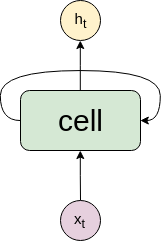
\includegraphics[scale=.5]{images/RNN.png} % Figure image
	\caption{RNN simple overview - feedback provides that the ouput (or a hidden layer) of the network, together with the new input at the current timestamp, is taken as input}
	\label{rnn} 
\end{figure}
Unpacked RNNs have the form of a chain of repeating nodes defined by very simple structure, Fig. \ref{rnn-unpacked} \cite{Olah_lstm}.
\begin{figure}
	\centering
	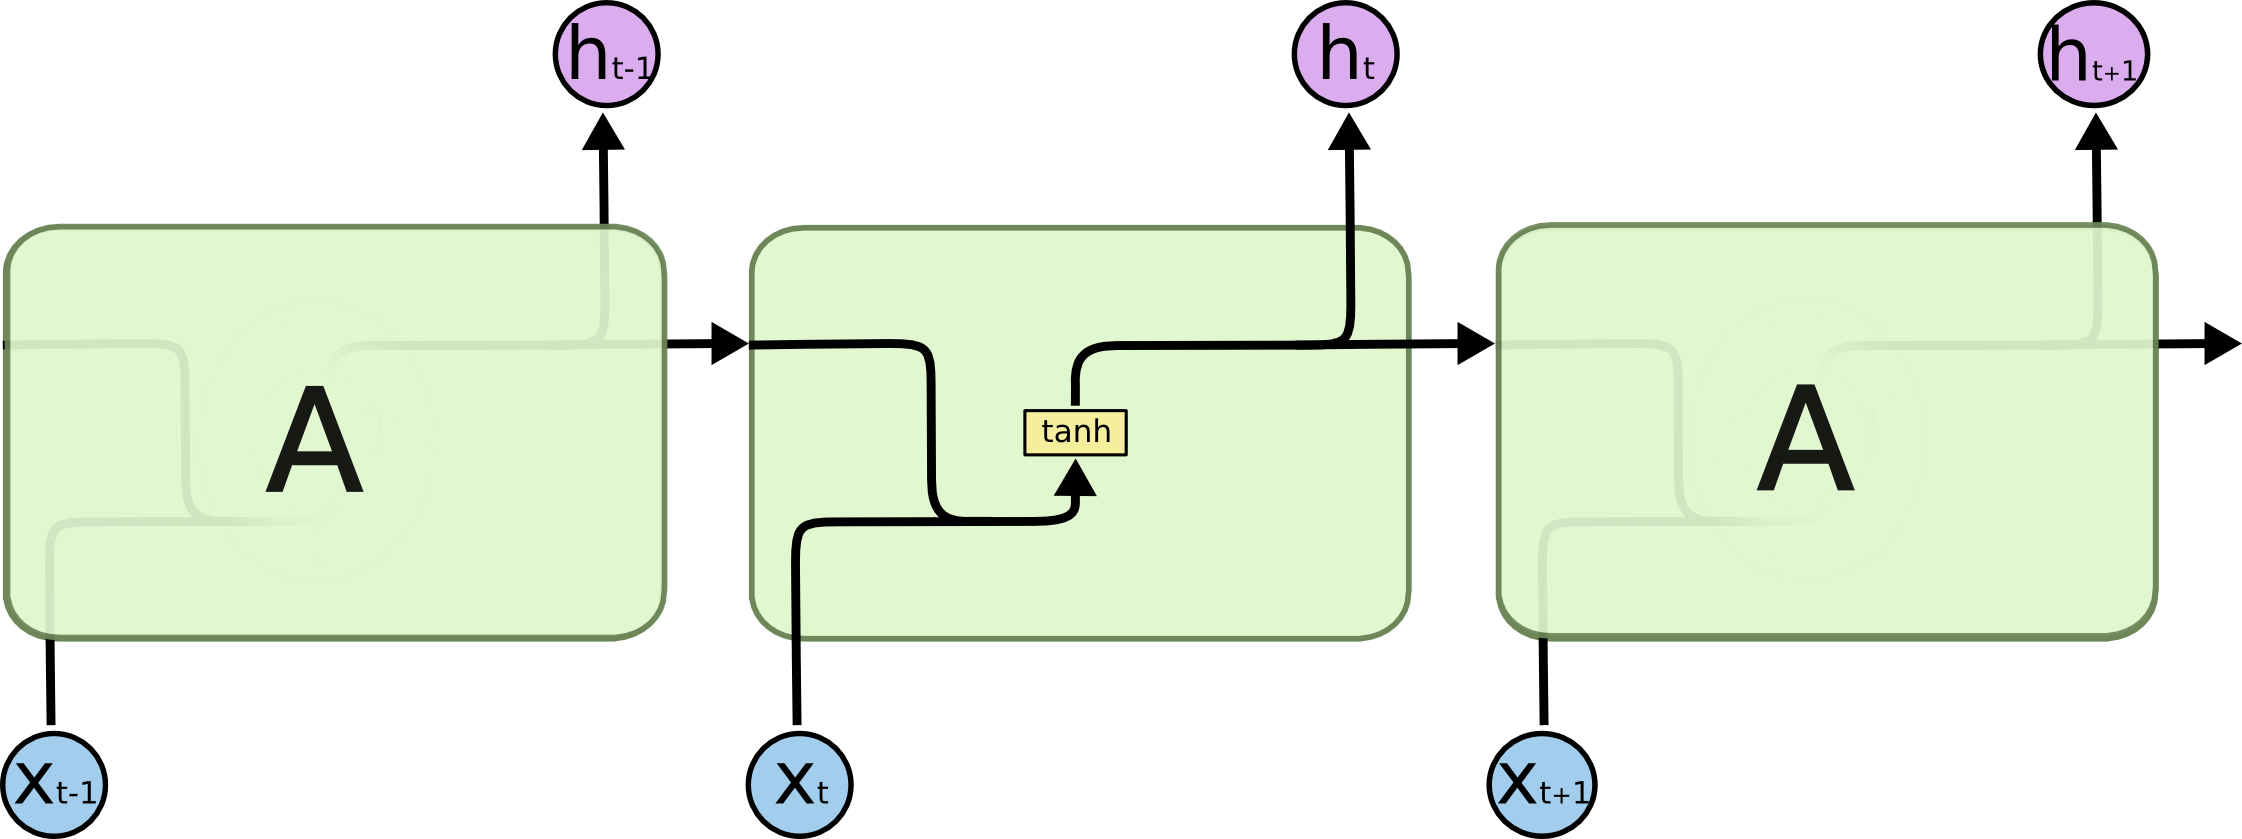
\includegraphics[scale=.5]{images/RNN-unpacked.png} % Figure image
	\caption{RNN are formed in a chain-like nature what makes them applicable for predicting future events of sequence data}
	\label{rnn-unpacked} 
\end{figure}

RNNs are using gradient descent (first-order iterative optimization algorithm, usually used for finding the minimum of a function) as a way to minimize the error caused by changing each weight in proportion the derivative of the error with respect to that weight. Problem with this approach is error gradient vanishing which is causing the RNN to become unable to learn to connect the information if the relevant data is devided by large gap. 
The problem of long-term dependencies is solved by applying Long Short-Term Memory network, LSTM for short, which are introduced by the Sepp Hochreiter and his team in 1997. in the \cite{Hochreiter_LSTM}. They proposed a model that is capable of remembering relevant information for long period of time and avoiding the long-term dependency issues. 

\section{Proposed LSTM model}

Just like the RNN, LSTM architecture is also formed as a chain structure. Difference is that every cell has four in-layers each performing specific operations on input data and interacting with others in a special way, general overview of LSTM network is shown on Fig. \ref{lstm}.
\begin{figure}
	\centering
	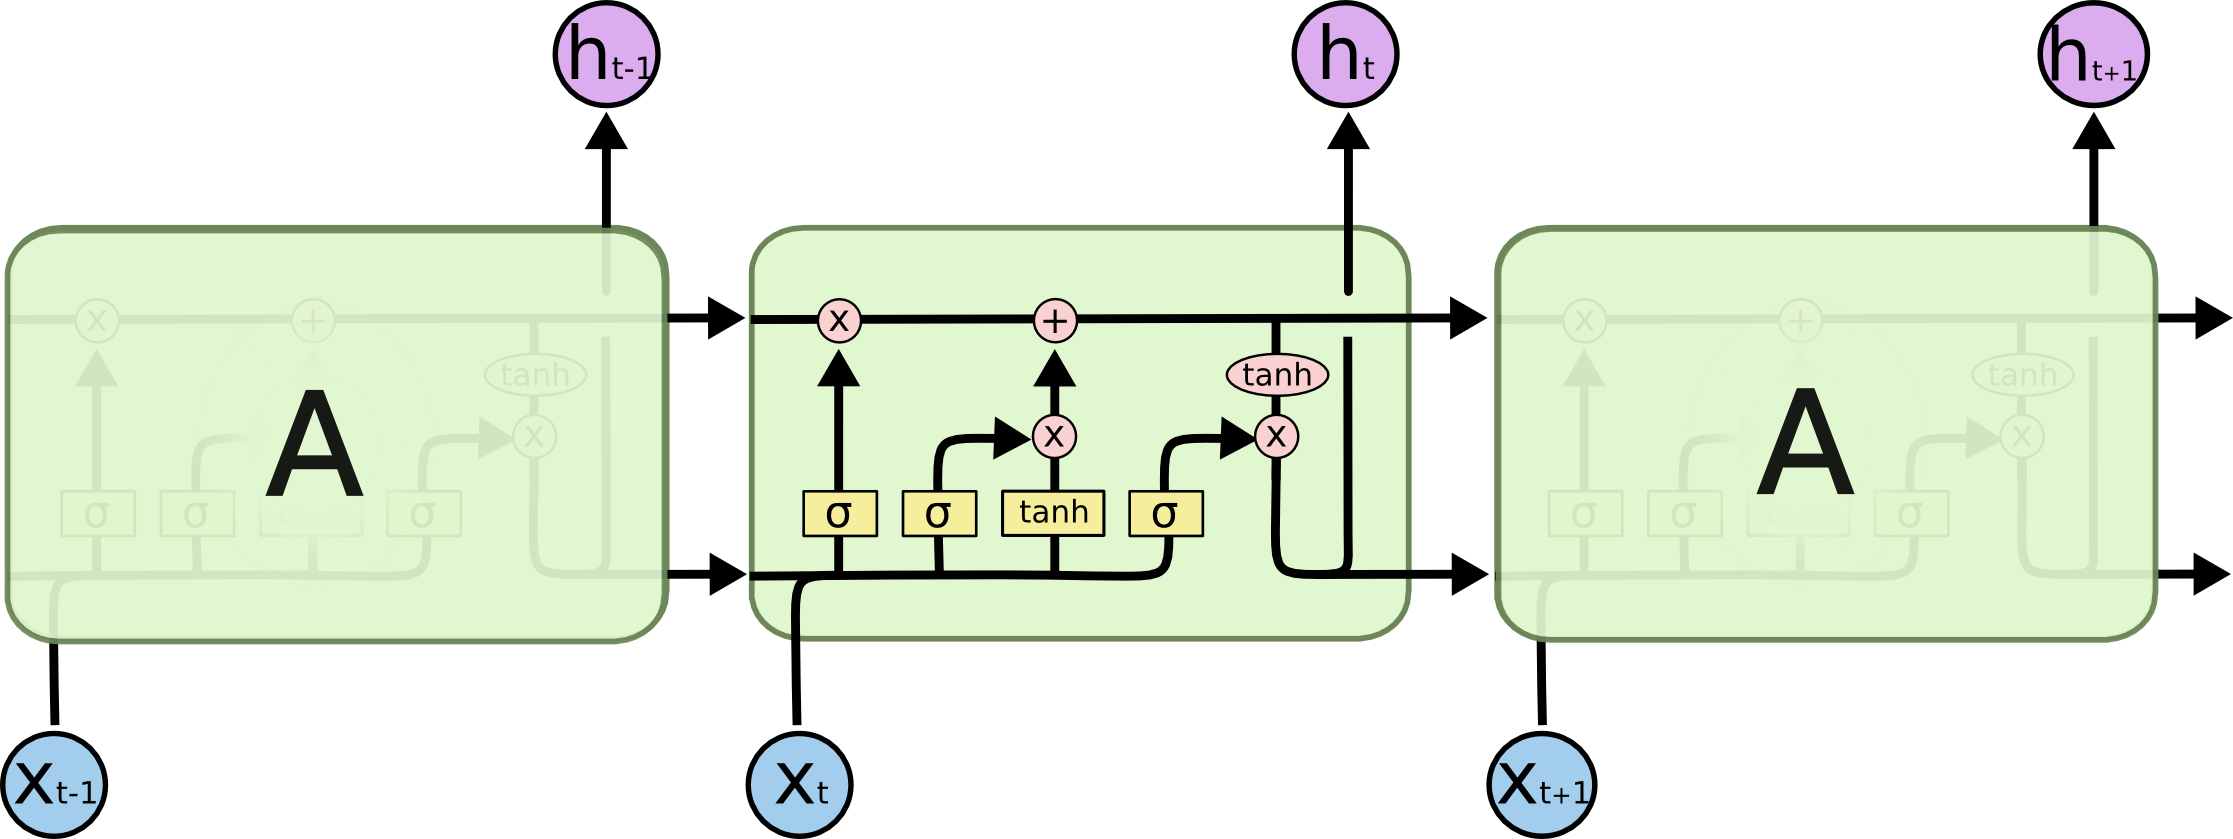
\includegraphics[scale=.4]{images/LSTM.png} % Figure image
	\caption{LSTM network preview}
	\label{lstm} 
\end{figure}

An LSTM cell is consisted of 5 components which allow it to model both long-term and short-term data:
\begin{itemize}
	\item cell state
	\item hidden state
	\item input gate 
	\item forget gate
	\item output gate 
\end{itemize}

Cell state, presented with the upper horizontal line in Fig. \ref{lstm}, runs through the whole cell and is affected by some minor linear changes.

Gates are the mechanism that allows information to be passed in selective fashion from the LSTM to the cell state. They consist of a sigmoid layer, which outputs value between 0 and 1 describing value of each component, and a multiplication operation.
There are three types of gates in LSTM network:
\begin{itemize}
	\item {Forget gate} - determines which information to remove from the cell state $$ f_{t} = \sigma (W_{f} \cdot [h_{t-1}, x_{t}] + b_{f}) $$
	\item {The second gate} - decides which new information should be written to the cell state. First, the sigmoid function decides which values to update and then the \emph{tanh} layer creates a vector of candidates to be added to the cell state. $$ i_{t} = \sigma (W_{i} \cdot [h_{t-1}, x_{t}] + b_{i}) $$ $$ C_{t} = tanh (W_{C} \cdot [h_{t-1}, x_{t}] + b_{C}) $$
	\item {The output gate} - decides what is going to be output of the concrete cell. The output is based on the filtered version of the cell state. $$ o_{t} = \theta (W_{o} [h_{t-1}, x_{t}] + b_{o}) $$ $$ h_{t} = o_{t} * tanh(C_{t})$$
\end{itemize}
%----------------------------------------------------------------------------------------
%	BIBLIOGRAPHY
%----------------------------------------------------------------------------------------

\printbibliography

%----------------------------------------------------------------------------------------

\end{document}
